% Document formatting:
\documentclass [11pt] {article}
\setlength {\parindent} {0pt}
\usepackage [margin = 1 in] {geometry}
\usepackage {hyperref}
\hypersetup {colorlinks=true, linkcolor=blue, filecolor=magenta, urlcolor=cyan}
\usepackage {graphicx}
\graphicspath { {img/} }
% Title:
\title {Mutual Exclusion Demonstration Write-Up}
\author {Jacob Naranjo, Tanush Samson, Alex Cadigan, Lionel Niyongabire}
% Builds document
\begin {document}
	\maketitle
	% Compiling and running
	\section {Compiling and Running}
	This program was tested on a laptop running MacOS.  These instructions for compiling and running the program are tailored for a MacOS environment.  These steps are not guaranteed to work on other systems.
	\begin {enumerate}
		\item Download \href {http://www.oracle.com/technetwork/java/javase/downloads/index.html} {Java}
  		\item \$ git clone https://github.com/AlexCadigan/MutualExclusionDemonstration.git
		\item \$ cd /MutualExclusionDemonstration/src/
		\item \$ javac MutualExclusionDemonstration.java Simulation.java Process.java
		\item \$ java MutualExclusionDemonstration
	\end {enumerate}
	% Description of program
	\section {Program Description}
	When the Mutual Exclusion Demonstration program is run, a GUI window will open asking for user input (Figure 1).\\  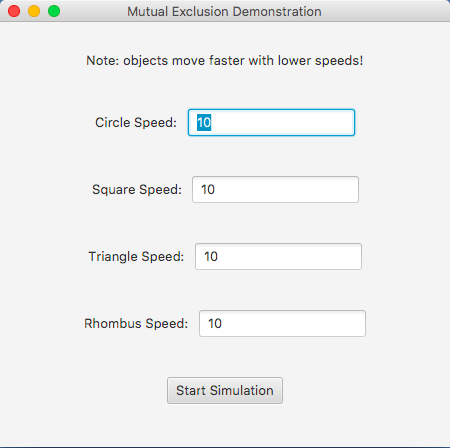
\includegraphics [scale = 1] {Figure1}\\\\  Figure 1 - Opening GUI window\\\\  In this first window, the user can select the speeds of the different objects.  The lower the speed, the faster the object will move.  When the user starts the simulation, a second GUI window will open, which will display the animation (Figure 2).\\\\  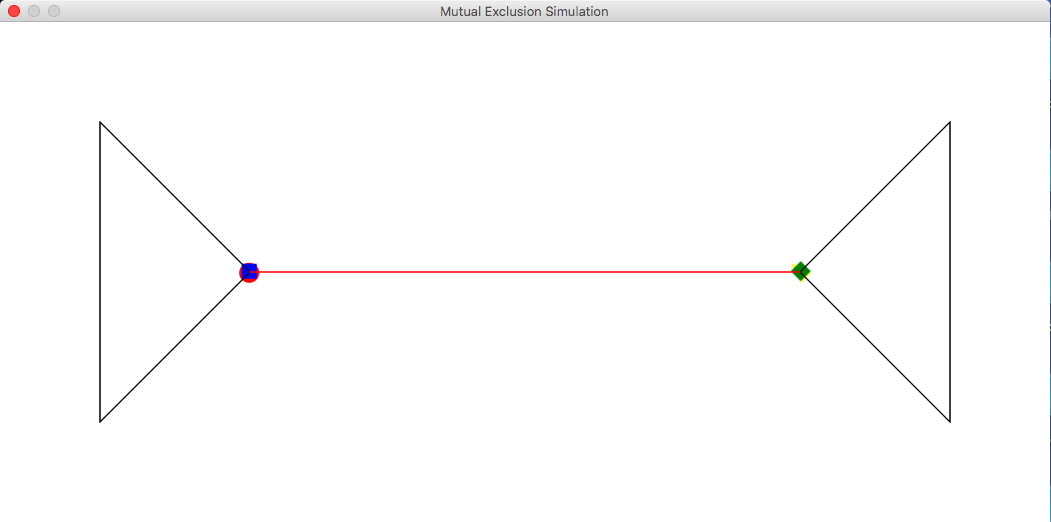
\includegraphics [scale = .5] {Figure2}\\  Figure 2 - Animation GUI window\\\\  The red path simulates the critical section of the distributed system, and the objects will first begin moving along the black paths (Figure 3).\\\\ 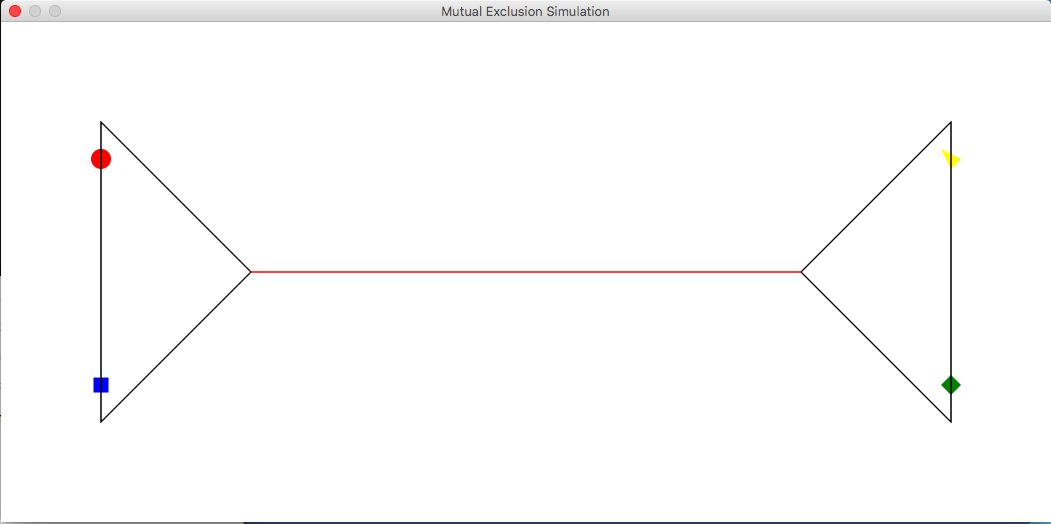
\includegraphics [scale = .5] {Figure3}\\ Figure 3 - Objects moving along the path\\\\  When an object reaches the intersection of the critical section, it will use Lamport's algorithm to determine if it may enter the critical section (Figure 4).\\\\  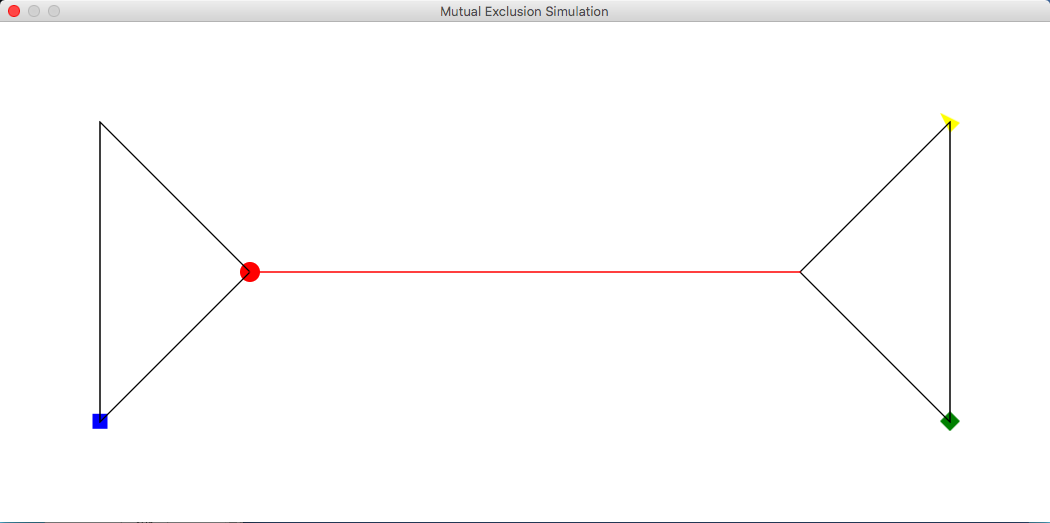
\includegraphics [scale = .5] {Figure4}\\ Figure 4 - An object at the critical section intersection\\\\  Lamport's algorithm consists of 5 steps:
	\begin {enumerate}
		\item When an object comes to the critical section, it sends a time-stamped request to every other object in the system and also enters the request in its local queue.
		\item When an object receives a request, it places it in its queue.  If the receiving object is not in the critical section, it sends a time-stamped acknowledgement message back to the sender.  Otherwise, it defers sending the acknowledgement message until it exits from the critical section.
		\item An object may enter the critical section when (1) its request is ordered ahead of all other requests (i.e., the time stamp of its own request is less than the time stamps of all other requests) in its local queue and (2) it has received acknowledgement messages from every other object in response to its current request.
		\item To exit from the critical section, an object (1) deletes the request from its local queue and (2) sends a time-stamped release message to all the other objects.
		\item When an object receives a release message, it removes the corresponding request from its local queue.
	\end {enumerate}
	See figure 5 for an example of an object entering the critical section.  Note that each object must wait to enter the critical section until there are no objects in the critical section.\\\\ 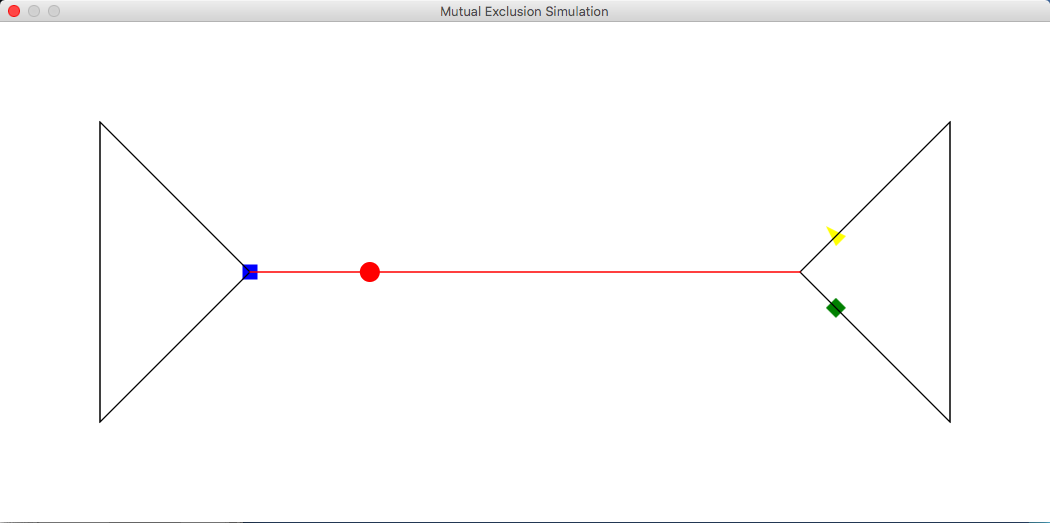
\includegraphics [scale = .5] {Figure5}\\ Figure 5 - An object moves through the critical section\\\\  The objects will continue moving until the user exits the GUI window.  All messages that are sent between objects are logged in a file for further analysis.  
	\section {Problems that Arose}
	\qquad The first problem that we encountered had to do with Java animations.  None of us had worked with Java animations before, so we had to research the libraries and classes provided in the JavaFX package.  We solved this problem by doing extensive research into the documentation behind JavaFX, and we built multiple small tests in order to learn how to use the functionality provided to us.  
	\paragraph {}
	\qquad The second major problem that we encountered was related to multithreading.  Originally, we attempted to implement the simulation by running each process independently on its own thread.  However, we had problems getting all of the threads to run at the same time.  Sometimes, all threads would run properly.  However, occasionally one or two of the threads would not run, and the simulation would not run properly.  After trying to debug the program and searching for the source of the error, we decided to abandon the multithreading implementation.  However, multithreading was not necessary to run the demonstration properly, and we were able to build a working program without the use of multiple threads.
	\paragraph {}
	\qquad The last major problem that we encountered stemmed from a misunderstanding of the project instructions and how distributed systems work in general.  Originally, we thought that a process should run continuously until it can be allowed into the critical section.  However, we realized that once a process had requested to enter the critical section, it was actually supposed to halt until it was allowed into the critical section.  We realized our mistake after we had already built a working version of the simulation.  As a results, we had to spend time refactoring our program in order to have it run properly.  However, refactoring gave us a chance to clean up our code and make it more structured, which ultimately benefited us.
	\paragraph {} 
	\qquad During the process of this project, we learned many interesting and important concepts related to our Distributed Systems class.  We learned how to build Java animations, which is an important skill that is very helpful in terms of visualizing algorithms.  We also learned the ins-and-outs of Lamport's Mutual Exclusion algorithm, which gave us a better understanding of how distributed systems work.  We also learned more about Java multithreading; a skill we will have to refine in the future.  It was very exciting to work with multithreading, because none of us had been exposed to very much multithreading in previous courses.  Overall, our understanding of the course material was improved while working on this project.
	\section {Overall Assessment}
	\qquad We would recommend this as an assignment to future classes.  We believe that this assignment would work well in the algorithms class and would give students an example of an algorithm for distributed systems.  However, this algorithm is more complex than many of the other algorithms students are exposed to, and we worry that the assignment may be too difficult for that level.  The assignment works very well in the distributed systems class.  It gives students a better understanding of how distributed systems work and an example of implementing an algorithm for distributed systems.  Therefore, we would recommend this assignment for future distributed systems classes.
\end {document}
